\documentclass{scrartcl}
\usepackage[T2A]{fontenc}
\usepackage[utf8]{inputenc}
\usepackage[russian]{babel}
\usepackage{graphicx}
\usepackage{amsmath}

\title{Усилитель мощности с контуром тока}
\author{}
\date{July 2016}

\begin{document}

\maketitle

\section{Постановка задачи}
Есть двигатель постоянного тока. Задача - разработать, собрать и протестировать устройство, позволяющиее реализовать контур тока применительно к этому двигателю. 
Желаемое время переходного процесса на застопоренном двигателе (без противо-ЭДС) -- не более 10мс. Интерфес связи с внешним управляющим контроллером -- SPI.

Параметры двигателя: максимальное напряжение $U_{max}$ 24В, рабочий ток до 5А.

\section{Железо}
\subsection{Струкутра системы}
В состав системы будут входить: 
\begin{enumerate}
    \item Силовая микросхема ключей, принимающая входной PWM сигнал и усиливающая его.
    \item Датчик тока.
    \item Управляющий микроконтроллер, реализующий обратную связь и закон управления.
\end{enumerate}


В качестве силового драйвера выбрана широкодоступная плата (\$18) от Pololu на базе микросхемы Freescale MC33926, максимальная частота ШИМ 20кГц, 5А в пике, коммутируемое напряжение от 5 до 28 вольт. 

Этот чип был взят за его возможность измерения абсолютной величины протекающего тока, которая в итоге не была использована. Таким образом, можно немного сэкономить, взяв более дешёвый драйвер со схожими характеристиками.

%http://www.robotshop.com/media/files/pdf/overview-1212.pdf

В качестве датчка тока выбран датчик Холла Allegro ACS714 (\$3), выдающий аналоговый сигнал с центром в 2.5В и 185мВ/А, типичная ошибка 1.5\%. На датчик была добавлена RC-цепочка в качестве фильтра низких частот с частотой среза 16кГц.

%http://www.microbot.it/documents/mr003-006_datasheet.pdf

В качестве управляющего микроконтроллера выбран ATMega328p, работающий на частоте 16МГц. Обвязка микроконтроллера -- китайский клон Arduino Nano v3 (\$1.5).

Микроконтроллер генерирует ШИМ сигнал через восьмибитный счётчик с делителем 8, таким образом, частота ШИМ сигнала $16\cdot 10^6 /255 /8 = 7.8$кГц, что укладывается в максимально доступные для драйвера 20кГц.

Делитель АЦП микроконтроллера установлен на 128; поскольку каждое измерение требует примерно 13 тактов, максимальная частота измерений протекающего тока равна примерно $16\cdot 10^6 / 128 / 13 = 9.6$кГц. Измерения производятся в фоновом режиме, извещая основную программу об окончании при помощи вызова соответствующего прерывания.

%http://www.atmel.com/images/Atmel-8271-8-bit-AVR-Microcontroller-ATmega48A-48PA-88A-88PA-168A-168PA-328-328P_datasheet_Complete.pdf

Отладочная информация передаётся микроконтроллером по интерфейсу SPI, для её записи был применён широкодоступный (\$10) китайский клон логического анализатора Saelae Pro 8 Logic.

Всё это было соединено вместе следующим образом:

\centerline{
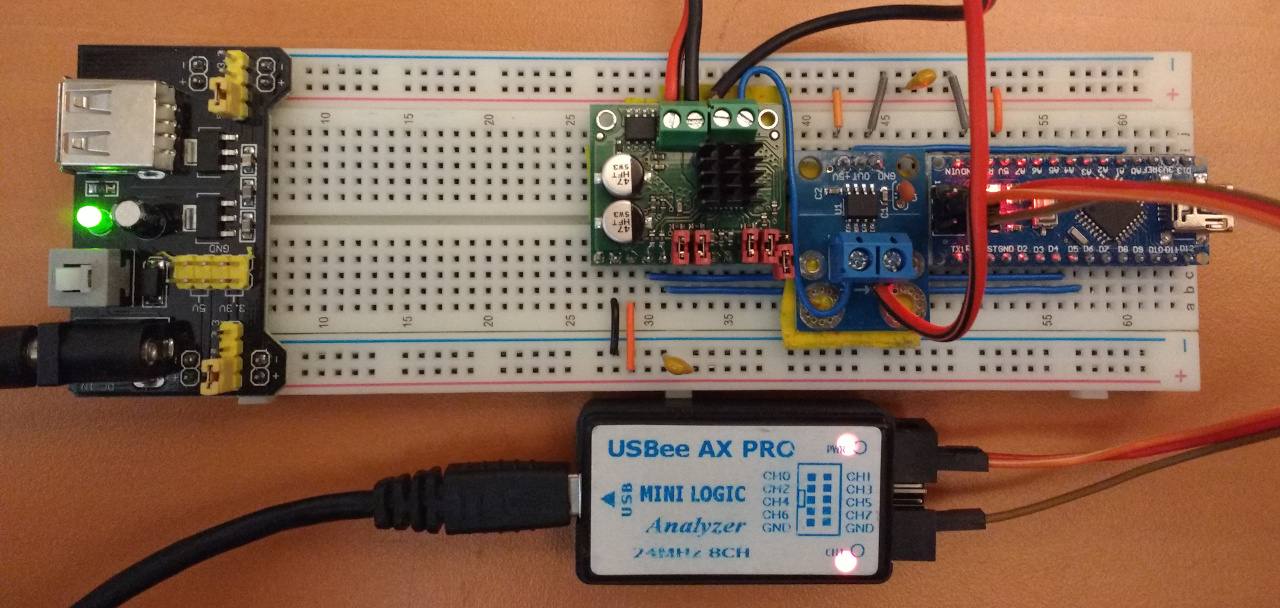
\includegraphics[width=.8\linewidth]{Fig/board.jpg}
}


\subsection{Проверка датчика тока}
Датчик тока был запитан от 4.96В источника, последовательно с датчиком был подключен резистор, через который было пропущено 2А. Теоретическое напряжение на выходном пине должно быть $4.96/2 + (2 \cdot 0.185 \pm 1.5\%$), измерение показало 2.84~В, что укладывается в расчётные параметры.
Затем было поменяно направление течения тока через резистор, при -2А
измеренное напряжение на выходном пине датчика составило 2.11В, что опять укладывается в расчётные параметры.
    
\centerline{
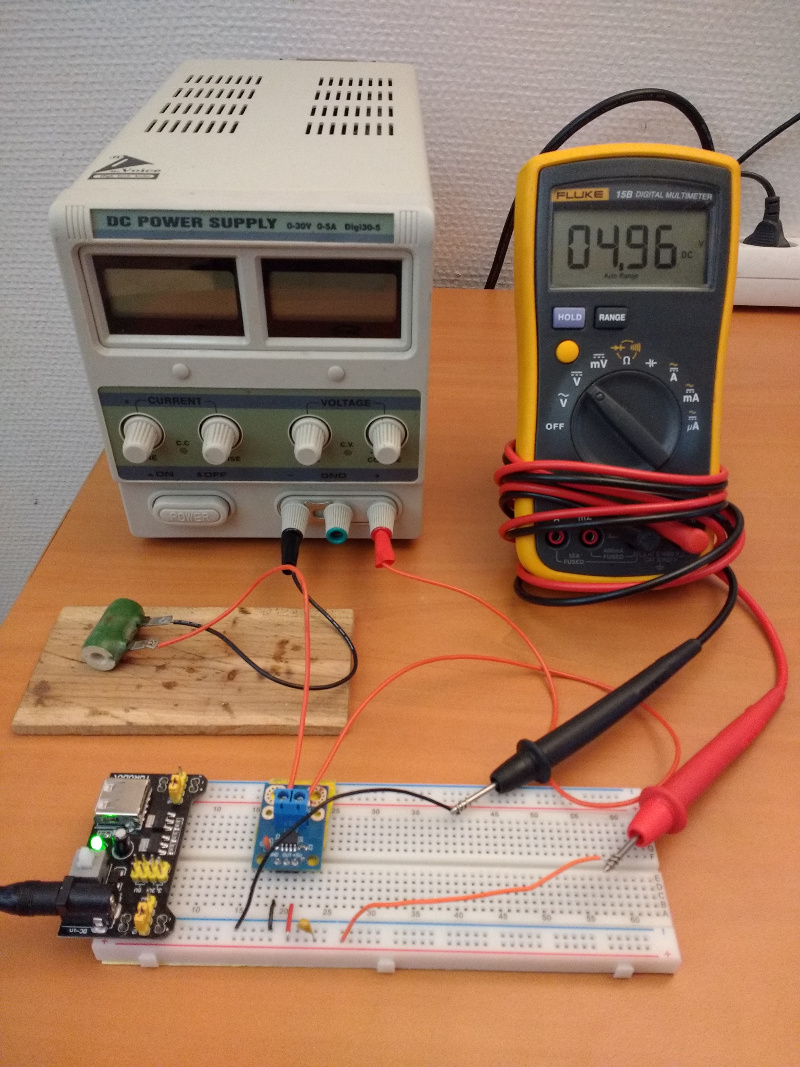
\includegraphics[width=.3\linewidth]{Fig/current_power.jpg}
%\hspace{.5cm}
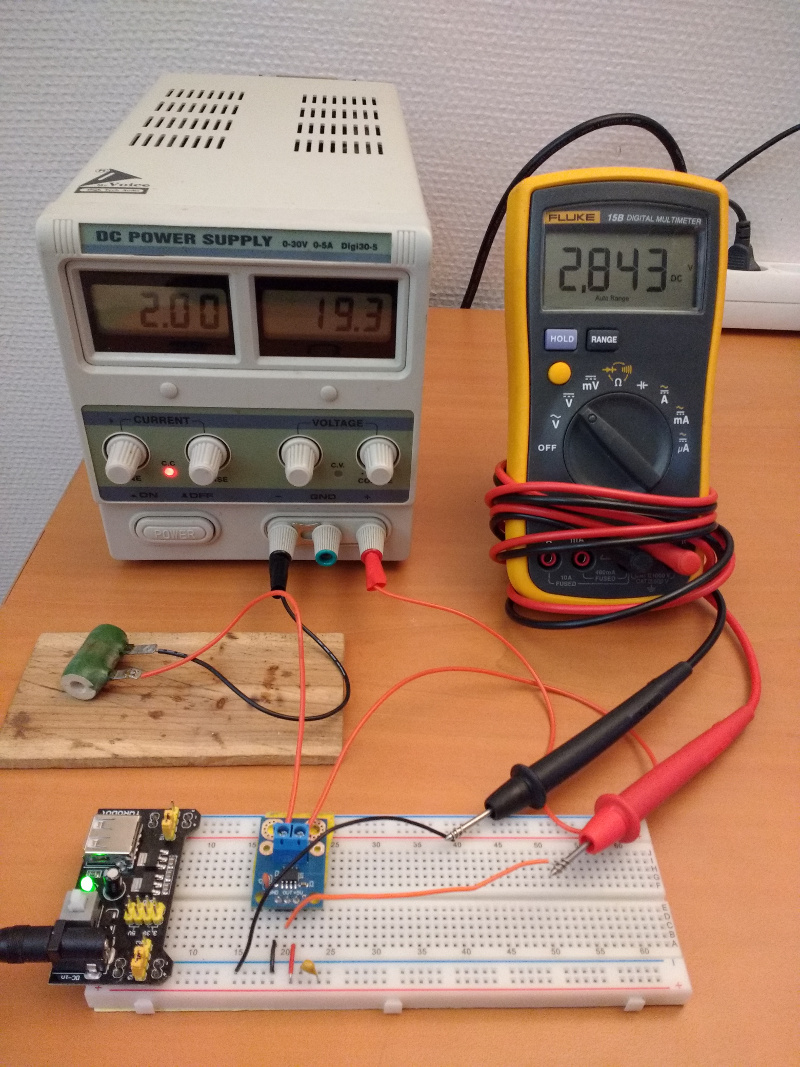
\includegraphics[width=.3\linewidth]{Fig/current_positive.jpg}
%\hspace{.5cm}
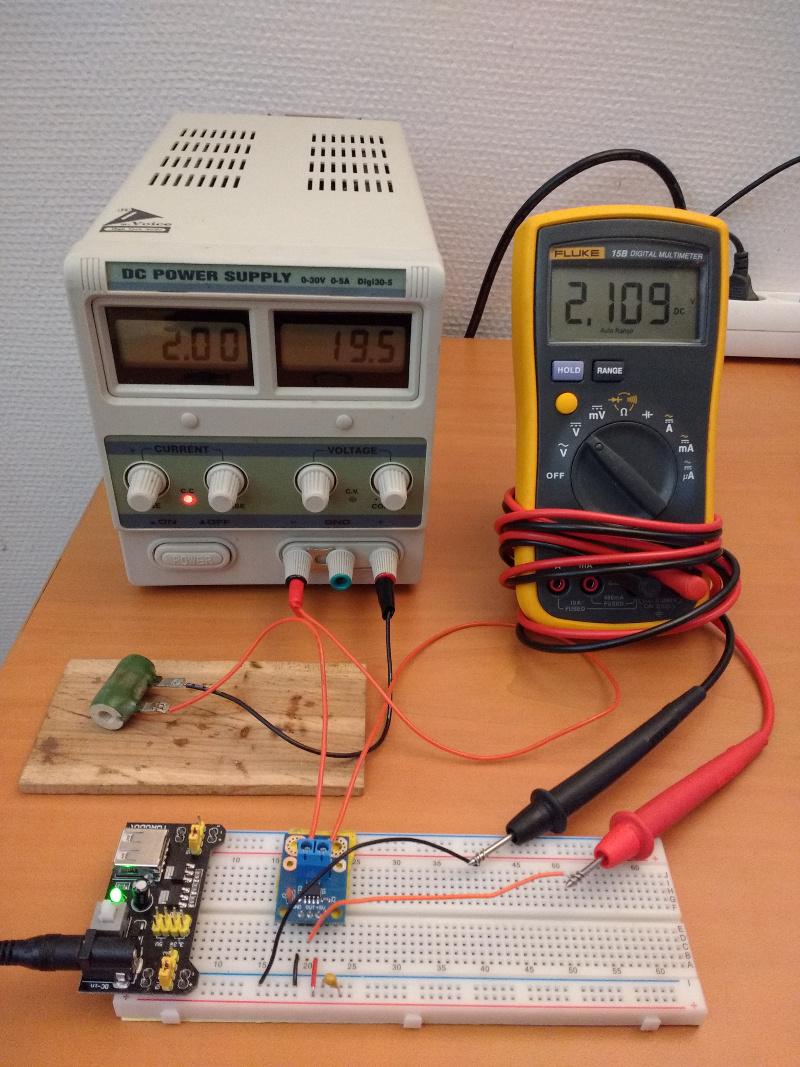
\includegraphics[width=.3\linewidth]{Fig/current_negative.jpg}
}

\section{Контур тока}
\subsection{Идентификация параметров}
Протекающие в двигателе процессы пописываются дифференциальным уравнением 
\[
    L \frac{dI}{dt}(t) = U(t) - RI(t) - C_\omega \omega(t),
\]
где $L$ -- индуктивность, $R$ -- сопротивление, $C_\omega$ -- коэффициент пртивоЭДС, $U(t)$ -- приложенное напряжение, $I(t)$ -- протекающий ток, $\omega(t)$ -- скорость вращения ротора. Для настройки контура тока мы зафиксируем ротор двигателя, то есть $\omega(t)\equiv 0$.

На следующей фотографии виден двигатель с заблокированным ротором, источник напряжения 24В, макет усилителя и подключенный логический анализатор для записи внутренних состояний регулятора.

\centerline{
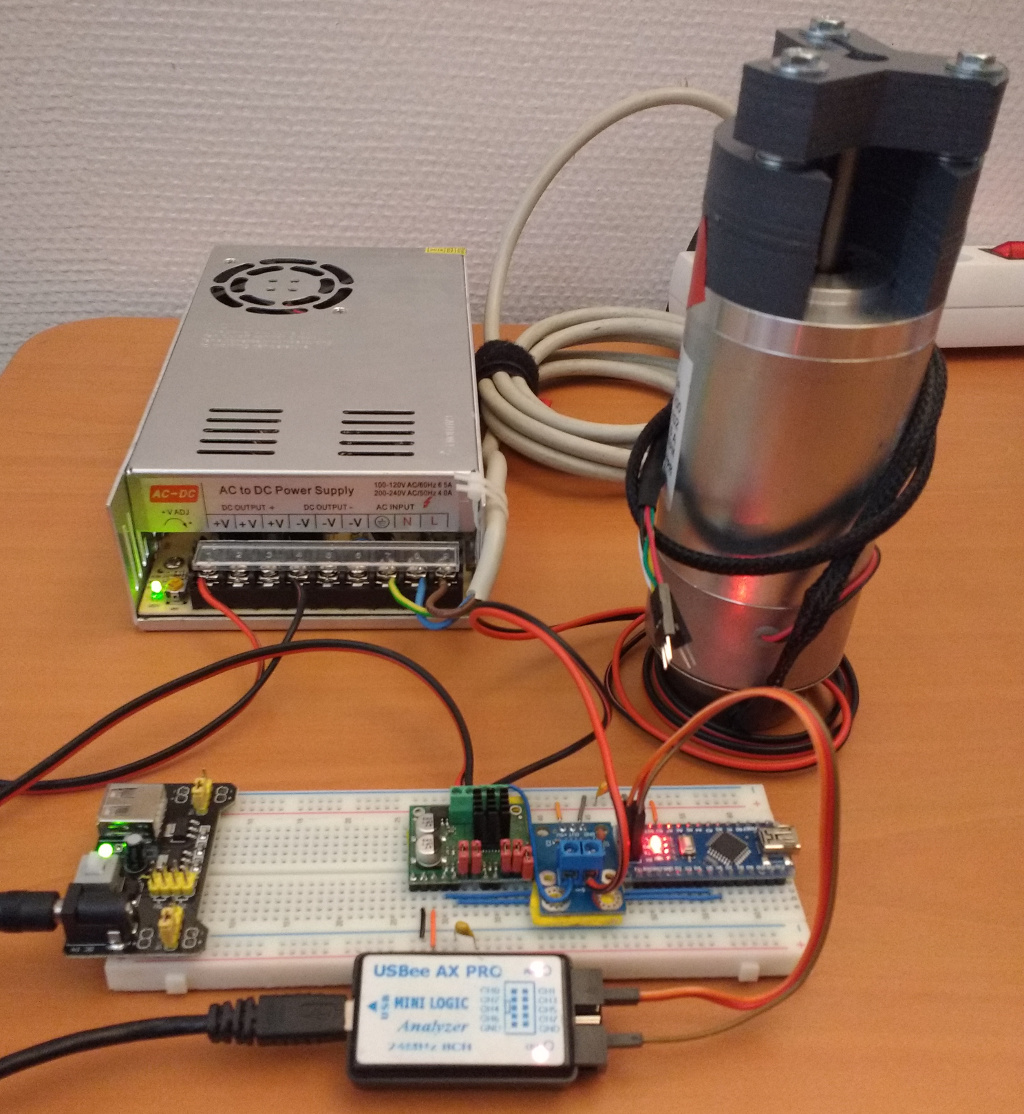
\includegraphics[width=.5\linewidth]{Fig/overall.jpg}
}


Передаточная функция двигателя от напряжения к току имеет вид
\begin{equation} \label{eq:TFCur}
    W(s) = \frac{1}{Ls + R} = \frac{K}{\tau s + 1}.
\end{equation}
Для построения системы управления током нас интересуют значения коэффициента передачи $K$ и постотянной времени $\tau$. 

Было проведено 11 экспериментов: три синусоидальных сигнала с частотами 61Hz, $\frac{1}{2}61$Hz и $\frac{1}{4}$61Hz и амплитудой 70\% от 24В, и меандр с периодом 0.128 секунды, скважностью 50\% и амплитудами 80\%, 60\%, 30\% и 10\% от 24В, в положительном и отрицательном направлениях. Пример реакции на синусоидальное напряжение и на меандр приведены на рисунке \ref{fig:OpenLoop}.
\begin{figure}
    \centering
    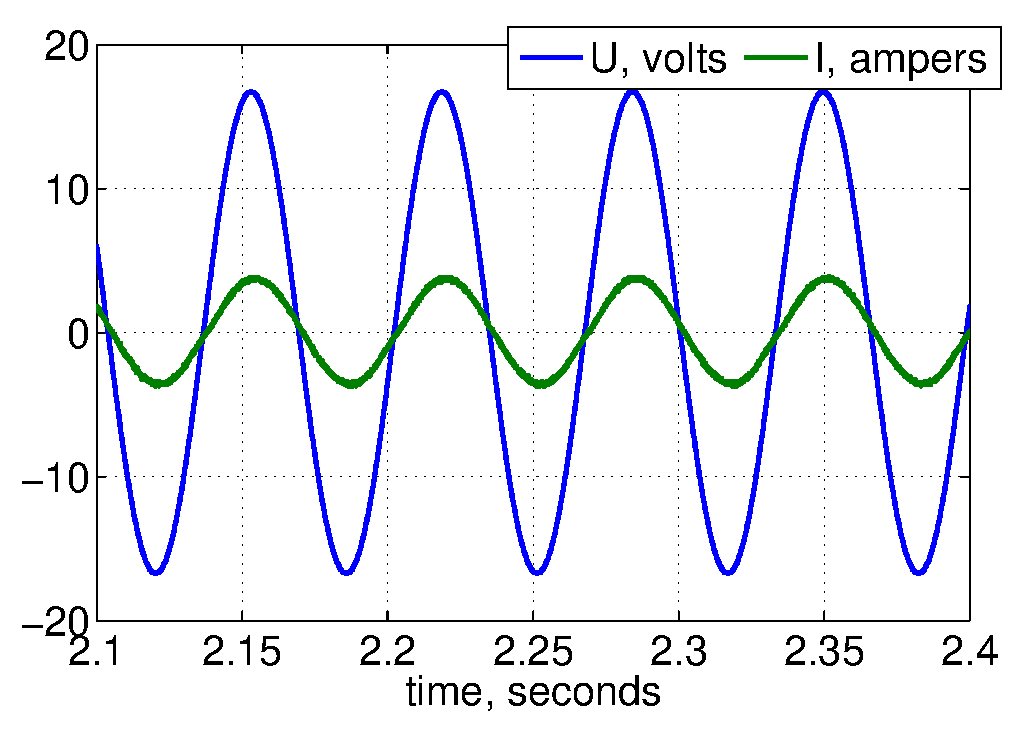
\includegraphics[height=.3\linewidth]{Fig/UIsin.eps} 
    ~
    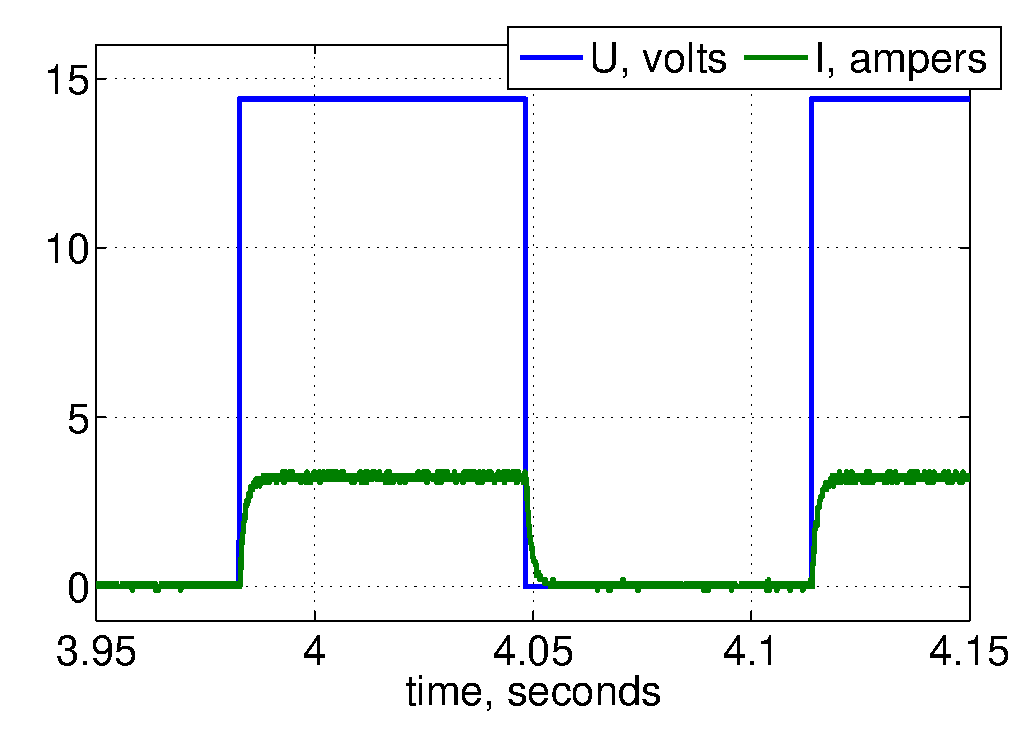
\includegraphics[height=.3\linewidth]{Fig/UIpulse.eps} 
    \caption{Сигнал тока при подаче входного сигнала в форме синусоиды и менадра, разомкнутый контур.}
    \label{fig:OpenLoop}
\end{figure}

По полученным экспериментальным данным с использованием функции \texttt{tfest} Matlab была получена оценка параметров передаточной функции \eqref{eq:TFCur}: $\hat{\tau}=0.0013$, $\hat{K}=0.22$. Степень совпадения с экспериментальными данными более 95\% для первых 7 экспериментов (амплитуда задания 60\% от максимума и выше), 86\% для экспериментов 8 и 9 (амплитуда задания 30\% от максимума) и 65\% для экспериментов 10 и 11. Предположительно, основной источник погрешности -- сэмплирование тока и мертвая зона драйвера силовых ключей.

\subsection{Расчёт регулятора}
Так как мы хотим получить апериодический характер переходных процессов в контуре тока, то желаемая передаточная функция замкнутого контура выбрана как
\[
    W_{cl}^\star(s) = \frac{1}{T_i s+1},
\]
где $T_i$ -- желаемая постоянная времени, выбранная как 2мс, что даст время переходного процесса $\approx 6$мс. Соответсвующая ей желаемая передаточная функция разомкнутого контура  
\[
    W_{ol}^\star(s) = \frac{1}{T_i s}.
\]

Исходя из желаемого передаточной функции разомкнутого контура, выберем передаточную функцию ПИ регулятора как
\[
    W_{PI}(s) = \frac{\hat{\tau}s+1}{\hat{K}Ts} = K_{P} + K_{I}\frac{1}{s},
\]
где $K_{P}=3$ и $K_{I}=2268$. 

Обозначим желаемое значение тока в обмотках как $I_\star(t)$. Тогда ошибка слежения по току $e_{I}(t):=I_\star(t) - I(t)$, а закон управления примет вид
\[
    U(t) = K_{P}e_{I}(t) + K_{I} \int_0^t{e_{I}(w)dw}.
\]

\subsection{Реализация}
регулятор тока был реализован в контроллере вот так.

\section{Проверка}
Проверка работы замкнутого контура была проведена для двух типов задания тока: синусоидального и меандра. На Рис. \ref{fig:ClosedLoop} приведены результаты работы регулятора для меандров большой амплитудой (4А) и малой (0.5А) амплитуды. Время переходного процесса составляет примерно 6мс.

Для дополнительноый проверки по экспериментальным данным была определена передаточная функция, описывающая замкнутый контур. Результат идентификации с помощью \texttt{tfest}:
\[
    \hat{W}_{cl}(s) = \frac{1}{0.0019s+1},
\]
что практически совпадает с желаемой передаточной функцией замкнутой системы. 

\begin{figure}
    \centering
    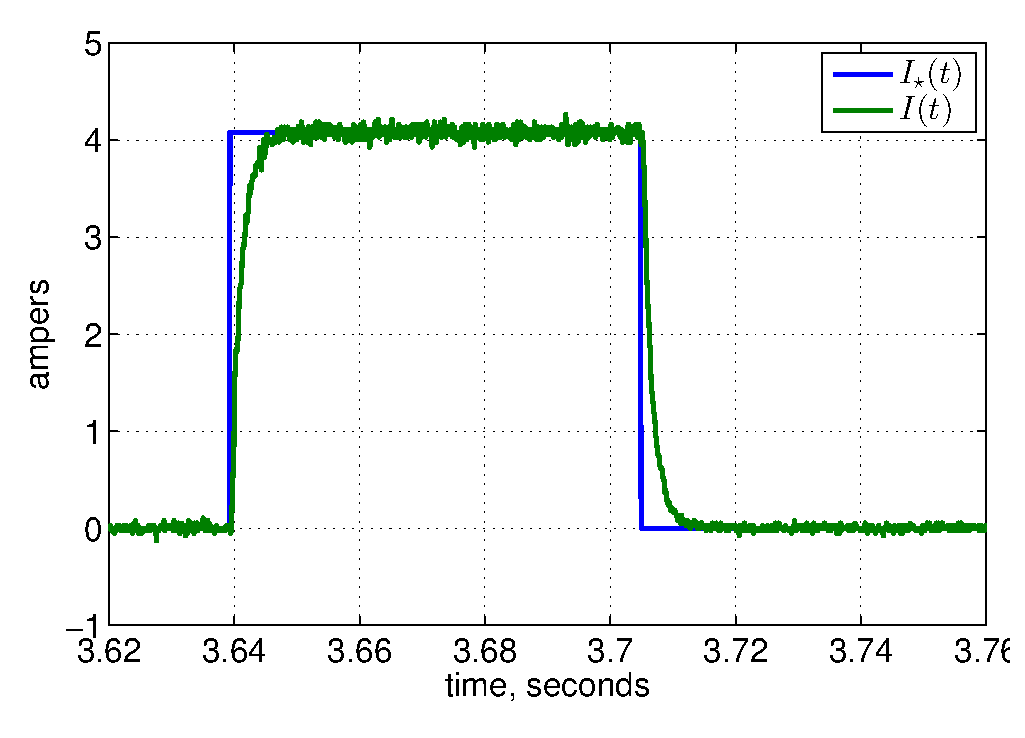
\includegraphics[height=.3\linewidth]{Fig/CL_meandr.eps} 
    ~
    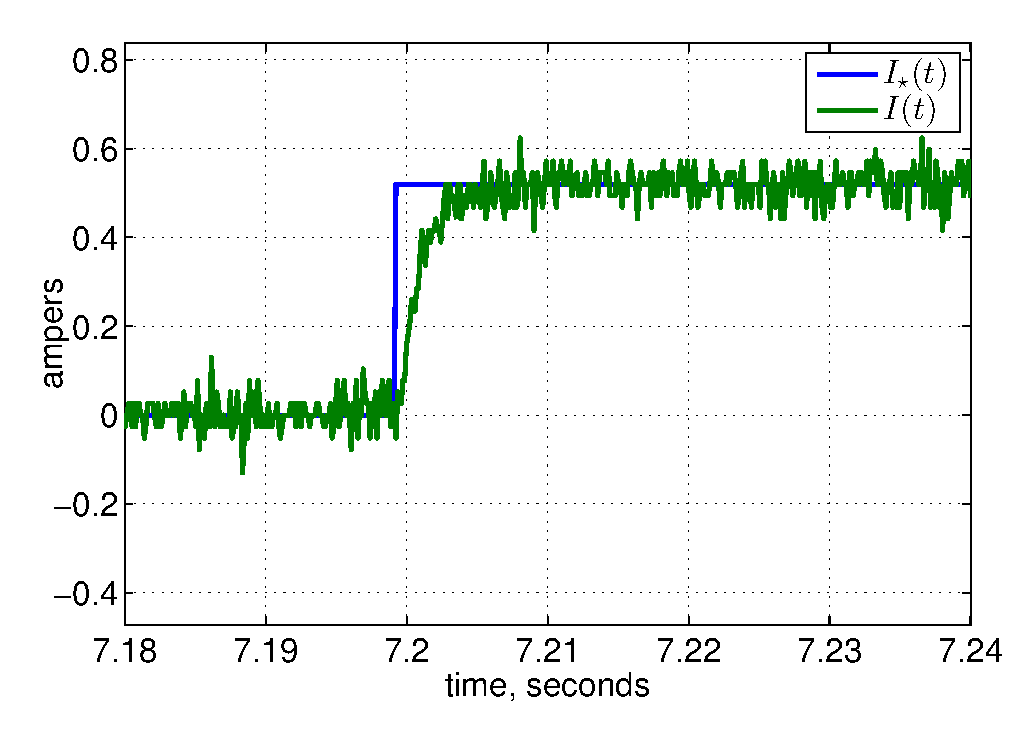
\includegraphics[height=.3\linewidth]{Fig/CL_meandr2.eps} 
    \caption{Задание по току и ток в замкнутой системе.}
    \label{fig:ClosedLoop}
\end{figure}

\section{Выводы}
Оставить это железо или менять.
\end{document}
